\documentclass[0-thesis.tex]{subfiles}

\begin{document}
The previous sections proposed the update architecture of the thesis, its key components,
and security considerations such as identity and access control. This section will discuss
a prototype implementation of the architecture as well as a manifest generator. 

\subsection{Manifest Implementation}
\label{ssec:manifest-implementation}
As manifests contain certain information difficult for humans to provide such as
monotonically increasing sequence numbers and digests, a manifest generator was created to
help test the prototype \parencite{manifest-generator}. It is a Python script which
accepts information about vendor and class namespace, version, image, and associated URL
in order to generate and format a manifest both in JSON and CBOR. The outputted manifest
follows the format specified in Section~\ref{ssec:manifest-format} and features all
required fields although many left blank. It is a bare-bones manifest containing only the
required information for a singular, monolithic update. There are no dependencies or
options. 

The manifest is a JSON map featuring the required elements shown in
Figure~\ref{fig:manifest-format}. The elements are in the same order as in the figure but
the names of the fields have been substituted for integers in order to save space.
Table~\ref{tab:manifest-substitution} shows this mapping. Nested structures such as
preconditions are described as an array of maps, where each map in the array constitutes
one precondition. The keys for these maps are also mapped to integers as in the main
manifest structure, resetting the counter for each nested structure. The mapping of keys
in nested structures is shown in Table~\ref{tab:nested-substitution}. Dependencies,
precursor image lists, URL/digest pairs, and options are described in the same way even
though the example manifest leaves most of these fields empty. The example manifest used
can be found in Appendix~\ref{app:manifest}. 

\begin{longtable}[]{@{}ll@{}}
    \caption{Mapping manifest elements to integers as keys in the JSON manifest.}
    \label{tab:manifest-substitution}\\
    \toprule
    Element name & Integer\tabularnewline
    \midrule
    \endhead
    versionID & 0\tabularnewline
    sequenceNumber & 1\tabularnewline
    preConditions & 2\tabularnewline
    postConditions & 3\tabularnewline
    contentKeyMethod & 4\tabularnewline
    payloadInfo & 5\tabularnewline
    precursorImage & 6\tabularnewline
    dependencies & 7\tabularnewline
    options & 8\tabularnewline
    \bottomrule
\end{longtable}

\begin{longtable}[]{@{}ll@{}}
    \caption{Mapping elements in nested structures to integers.}
    \label{tab:nested-substitution}\\
    \toprule
    Element name (corresponding structure) & Integer\tabularnewline
    \midrule
    \endhead
    type (conditions and options) & 0\tabularnewline
    value (conditions and options) & 1\tabularnewline
    \bottomrule
    URL (URL/digest pair) & 0\tabularnewline
    digest (URL/digest pair) & 1\tabularnewline
    \bottomrule
    format (payload info) & 0\tabularnewline
    size (payload info) & 1\tabularnewline
    storage (payload info) & 2\tabularnewline
    URL/digest pair (payload info) & 3\tabularnewline
    \bottomrule
\end{longtable}

% TODO: Show pieces of manifest implementation


\subsection{Prototype Implementation}
\label{ssec:prototype-implementation}
% TODO: Overview of prototype: what it includes, protocols, largely how it works, assumptions
The prototype used in the thesis is developed in order to measure the efficiency of
transport during an update procedure. It consists of a server and a client both
implemented in Contiki-NG. The prototype uses a pull model meaning the client running on a
board initiates the update procedure and the server responds with its resources. The
server is implemented in Contiki-NG as a proof-of-concept that a more capable IoT device
could be used as an update server.

% TODO: Check what I've already written about COSE in Contiki-NG (previous section)
% TODO: Double check what an AAD is/does
The prototype makes use of CoAPs over DTLS with COSE encryption of payloads. Ideally COSE
would be used for signing payloads as confidentiality is provided by DTLS, but COSE
implementations in Contiki-NG are limited and at the time of development did not support
signing. Implementing COSE signing would prove too time consuming for a project of this
scope, thus COSE encryption is used instead as a proof-of-concept of using COSE in the
update architecture. Encrypting via COSE requires more information than signing such as
keys, nonces, and AADs, these have been hard-coded into the client and server. Furthermore
certificate support in Contiki-NG is lacking and the prototype thus uses hard-coded
pre-shared keys in order to use DTLS. The last assumptions made are about the files being
transfered. The prototype and evaluation only makes use of one certificate and firmware
image, thus sizes of buffers in the client have been statically allocated in order to make
implementation easier. In reality with manifests and images of varying sizes, dynamic
memory allocation would be needed in order to accept varying updates.

The interactions of the client and server are simplistic and the client has no other
behaviour than to initiate and complete the update procedure. As shown in
Figure~\ref{fig:client-server-interaction}, the interaction starts with a POST request
from the client to the registration endpoint of the server. The registration is sent as a
confirmable CoAP packet and is thus acknowledged by the server. Afterwards, the client
sends a GET request for a manifest. The idea is that the endpoint \texttt{update/manifest}
is a well known endpoint just like \texttt{update/register} and all devices in the network
register and poll for manifests at these endpoints. Upon a request to
\texttt{update/manifest} it is up to the server to decide whether there is a suitable
manifest or not, offloading any decision making from the device. Since the prototype only
makes use of one manifest such logic is not implemented, but in real deployments the
\texttt{update/manifest} server resource would handle that by using the information from
the devices' profile.

\begin{figure}
    \caption{The interactions of client and server during an update procedure.}
    \label{fig:client-server-interaction}
    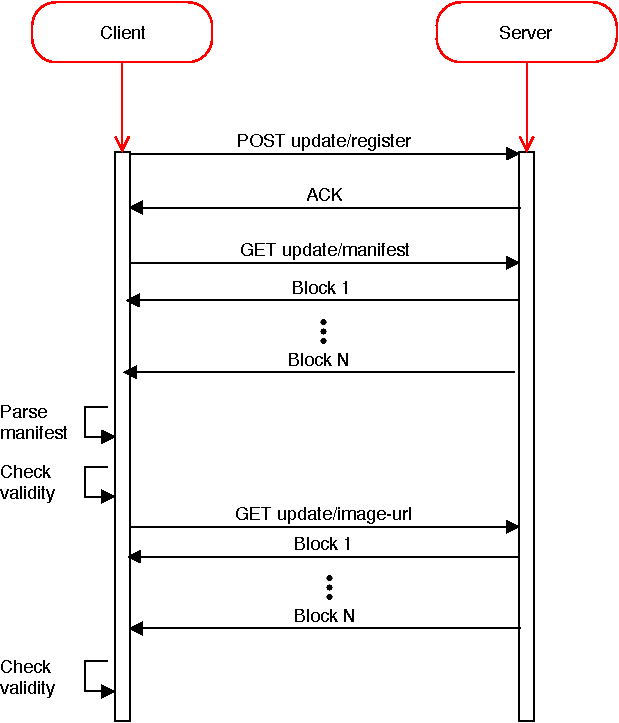
\includegraphics{images/client-server-sequence.pdf}
\end{figure}

If the server finds a suitable manifest, it encodes and encrypts it using COSE and then
sends it through CoAPs' block option. The reasoning for encrypting the entire payload at
once instead of each block is that encrypting each block would not add any security as it
uses the same key. By encrypting the entire payload once it will only be decrypted once,
saving the client from running cryptographic functions many times. After the client has
reassembled the manifest it decrypts and decodes it, and then runs a simple parser. After
parsing is done the client must check the preconditions to make sure it is the intended
recipient by comparing vendor and class IDs, and any other custom logic.

If the client deems the manifest to be valid it requests the update image from the URL
specified in the manifest. The endpoint is now specific for this particular class of
device and version and is not known in advance, it must be in the manifest. The image,
also too large for a single CoAP message, is encoded, encrypted, and transferred in
blocks. When the client has received and decrypted the image, it calculates the SHA-256
hash of it, comparing it to the hash contained in the manifest. This concludes the
transfer of an update.

\subsubsection{Server Specifics}
\label{sssec:server-specifics}
% TODO: Talk more in detail about how the server and its resources are implemented

\subsubsection{Client Specifics}
\label{sssec:client-specifics}
% TODO: Talk more in detail about the client: register and manifest from known endpoints,
% parsing manifest (show structure here?), checking manifest and custom logic, decoding
% payloads
In the client code, the manifest is received as a string, still formatted as JSON. In
order to parse it, structs resembling the format of the manifest were created. Nested
elements such as preconditions are implemented as linked lists, where each precondition
contains a type, a value, and a pointer to the next. The manifest structure contains a
pointer to the first precondition, from which the entire set of preconditions can be
retrieved. The set of structs and their relations are as in
Figure~\ref{fig:manifest-format}, where conditions, URL/digest pairs, and options are
implemented in a linked list way. This kind of structuring is extensible, allowing
implementers to easily add new conditions or options as well as specify an arbitrary
amount of dependencies, precursors, and mirrors of images.




\end{document}